\begin{figure}[!htb]
\begin{center}
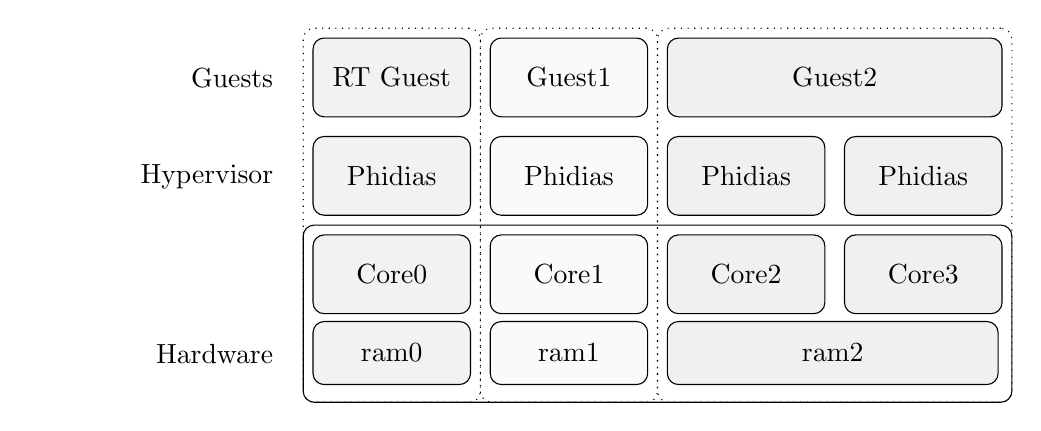
\begin{tikzpicture}

\node at (0,0)[rectangle, draw=black, fill=black!5, rounded corners, minimum height = 1cm, minimum width = 2cm, anchor=south west] (core0) {Core0};
\node at (2.25,0)[rectangle, draw=black, fill=black!2, rounded corners, minimum height = 1cm, minimum width = 2cm, anchor=south west] (core1) {Core1};
\node at (4.50,0)[rectangle, draw=black, fill=black!6, rounded corners, minimum height = 1cm, minimum width = 2cm, anchor=south west] (core2) {Core2};
\node at (6.75,0)[rectangle, draw=black, fill=black!6, rounded corners, minimum height = 1cm, minimum width = 2cm, anchor=south west] (core3) {Core3};

\node at (0,-0.9) [rectangle, draw=black, fill=black!5, rounded corners, minimum height = 0.8cm, minimum width = 2cm, anchor=south west] (ram0) {ram0};
\node at (2.25,-0.9) [rectangle, draw=black, fill=black!2, rounded corners, minimum height = 0.8cm, minimum width = 2cm, anchor=south west] (ram1) {ram1};
\node at (4.50,-0.9) [rectangle, draw=black, fill=black!6, rounded corners, minimum height = 0.8cm, minimum width = 4.2cm, anchor=south west] (ram2) {ram2};

\begin{scope}[fill opacity=0.0]
\node at (-0.125,-0.125-1)[rectangle, draw=black, fill=white, rounded corners, minimum height = 2.25cm, minimum width = 9.00cm, anchor=south west] (hardware) {};

\node at (-0.125,-1.125)[rectangle, draw=black, fill=black!5, dotted, rounded corners, minimum height = 4.75cm, minimum width = 2.25cm, anchor=south west] (rtg) {};
\node at (2.125,-1.125)[rectangle, draw=black, fill=black!2, dotted, rounded corners, minimum height = 4.75cm, minimum width = 2.25cm, anchor=south west] (g1) {};
\node at (4.375,-1.125)[rectangle, draw=black, fill=black!6, dotted, rounded corners, minimum height = 4.75cm, minimum width = 4.50cm, anchor=south west] (g2) {};

\end{scope}

\node at (0.0,1.25)[rectangle, draw=black, fill=black!5, rounded corners, minimum height = 1cm, minimum width = 2cm, anchor=south west] {Phidias};
\node at (2.25,1.25)[rectangle, draw=black, fill=black!2, rounded corners, minimum height = 1cm, minimum width = 2cm, anchor=south west] {Phidias};
\node at (4.50,1.25)[rectangle, draw=black, fill=black!6, rounded corners, minimum height = 1cm, minimum width = 2cm, anchor=south west] {Phidias};
\node at (6.75,1.25)[rectangle, draw=black, fill=black!6, rounded corners, minimum height = 1cm, minimum width = 2cm, anchor=south west] {Phidias};

\node at (0.0,2.5)[rectangle, draw=black, fill=black!5, rounded corners, minimum height = 1cm, minimum width = 2cm, anchor=south west] {RT Guest};
\node at (2.25,2.5)[rectangle, draw=black, fill=black!2, rounded corners, minimum height = 1cm, minimum width = 2cm, anchor=south west] {Guest1};
\node at (4.50,2.5)[rectangle, draw=black, fill=black!6, rounded corners, minimum height = 1cm, minimum width = 4.25cm, anchor=south west] {Guest2};

\node (hardware) at (-2.0, -0.5) [text width=3cm, align=right]{Hardware};
\node (phidias) at (-2.0, 1.75) [text width=3cm, align=right]{Hypervisor};
\node (guests) at (-2.0, 3.0) [text width=3cm, align=right]{Guests};

\end{tikzpicture}
\end{center}
\ifreport
\caption{Example partitioning of a multicore x86 platform using Phidias. The guest are allocated separate CPU cores and RAM memory. 
Since Phidias follows multikernel design approach, a clone of Phidias runs on each core.}
\fi
\label{fig-static-part}
\end{figure}
